\def\CTeXPreproc{Created by ctex v0.2.9, don't edit!}
%\documentclass{beamer}
\documentclass[%handout,
xcolor=pdftex]{beamer}
\mode<presentation> {
  \usetheme{Warsaw}
  \setbeamercovered{transparent}
}
\let\Tiny=\tiny
\usetheme{Singapore}
\usecolortheme{dolphin}
\usepackage{amsmath}
\usepackage{textcomp}
\usepackage{amssymb}
\usepackage{amsthm}
\usepackage{graphicx}
\usepackage{color}
\usepackage{lipsum}
\usepackage{hyperref}
\usepackage{multirow}
\usepackage{bm}
\DeclareMathSymbol{\Phi}{\mathalpha}{operators}{8}
%\setbeamertemplate{headline}{}
\setbeamertemplate{footline}[page number]
\newcommand\Fontvi{\fontsize{9pt}{8}\selectfont}
\newcommand\Fontvii{\fontsize{7pt}{8}\selectfont}
\newcommand{\backupbegin}{
   \newcounter{finalframe}
   \setcounter{finalframe}{\value{framenumber}}
}
\newcommand{\backupend}{
   \setcounter{framenumber}{\value{finalframe}}
}\newtheorem{proposition}{Proposition}
\title{Unit 15: Seasonal ARMA Models}
\author[STAT 5170: Applied Time Series, Unit 15]{Taylor R. Brown}
\institute{Department of Statistics, University of Virginia}
\date{Fall 2020}

\AtBeginSubsection[] {
  \begin{frame}<beamer>{Outline}
    \tableofcontents[currentsection,currentsubsection]
  \end{frame}
}



\begin{document}


\frame{\titlepage}


\begin{frame}
\frametitle{Readings for Unit 15}

Textbook chapter 3.9 page 148 to 151 (example 3.47).

\end{frame}



\begin{frame}
\frametitle{Last Unit}
\begin{enumerate}
\item Integrated models for nonstationary data.
\item Building ARIMA models (Exploratory data analysis, Model estimation, Model diagnostics, Model selection).
\end{enumerate}
\end{frame}

\begin{frame}
\frametitle{This Unit}

Seasonal ARMA models for seasonal time series.


\end{frame}


\begin{frame}
\frametitle{Motivation}

So far, we've avoided seasonal data. The ARIMA models that we've discussed do not account for seasonality. However, we may wish to have a model for monthly observations which depends on both the previous month and the same month one year ago. SARMA models will allow us to do that.

\end{frame}

\section{SARMA Model}
\frame{\tableofcontents[currentsection]}

\begin{frame}
\frametitle{SARMA Model}

We can write the pure seasonal ARMA model, ARMA$(P,Q)_s$, using backshift operators in the following way.
\begin{equation}
\Phi_P (B^s) x_t =\Theta_Q(B^s) w_t
\end{equation}
where
$$
\Phi_P(B^s)=1-\Phi_1 B^s-\Phi_2B^{2s}-\cdots-\Phi_P B^{Ps}
$$
and
$$
\Theta_Q(B^s)=1+\Theta_1 B^s+\Theta_2B^{2s}+\cdots+\Theta_Q B^{Qs}.
$$
The first polynomial is the seasonal autoregressive operator and the second is the seasonal moving average operator.



\end{frame}

\begin{frame}
\frametitle{Seasonal ARMA Model}

Suppose you have quarterly data and want to think about an ARMA$(1,1)_4$.  This would be
$$
(1-\Phi_1 B^4) x_t=(1+\Theta_1 B^4) w_t
$$
or
$$
x_t=\Phi_1 x_{t-4}+w_t+\Theta w_{t-4}.
$$
This is essentially an ARMA model, except lags between zero and four are omitted.

\end{frame}

\begin{frame}
\frametitle{Seasonal ARMA Model}

Just like the nonseasonal ARMA models, the pure seasonal ARMA$(P,Q)_s$ is causal only when the roots of $\Phi_P(z^s)$ lie outside the unit circle, and is invertible only when the roots of $\Theta_Q(z^s)$ lie outside the unit circle.
\end{frame}

\section{Exploratory Data Analysis}
\frame{\tableofcontents[currentsection]}

\begin{frame}
\frametitle{ACF for Seasonal MA}

Let's consider monthly data and look at a seasonal MA(1).  The model would be written as
$$
x_t=w_t+ \Theta_1 w_{t-12}.
$$
The variance will be $\sigma_w^2(1+\Theta_1^2)$.

\end{frame}

\begin{frame}
\frametitle{ACF for Seasonal MA}

The autocovariance would then be (for $h>0, h\neq12$)

\vspace{50mm}

\end{frame}

\begin{frame}
\frametitle{ACF for Seasonal MA}

However, when $h=12$,

\vspace{50mm}

\end{frame}

\begin{frame}
\frametitle{ACF for Seasonal MA}

In general, for the MA$(Q)_s$ model
$$
x_t = w_t + \Theta_1 w_{t-s} + \Theta_2 w_{t-2s} + \cdots + \Theta_Q w_{t-Qs},
$$
\begin{itemize}
\item[$\bullet$] $\gamma(h)=0$ for $h\ne ks, k=1,2,\ldots.$
\item[$\bullet$] $\gamma(0),\gamma(s),\gamma(2s),\ldots,\gamma(Qs)$ are non-zero.
\item[$\bullet$] $\gamma(ks)=0$ for $k\ge Q+1$.
\end{itemize}

\end{frame}

\begin{frame}
\frametitle{ACF for Seasonal AR}

Now, let's think about a pure seasonal AR$(1)_{12}$ process.  This would be
$$
x_t= \Phi_1 x_{t-12}+w_t.
$$

Iterate recursively to obtain
$$
x_t= \sum_{k=0}^\infty \Phi_1^k w_{t-12k}
$$
for $|\Phi_1|<1$.
\end{frame}

\begin{frame}
\frametitle{ACF for Seasonal AR}

The autocovariance would then be (for $h>0, h\neq12k$)

$$
\gamma(h)=E(x_t x_{t-h})=E\left[ \Big ( \sum_{k=0}^\infty \Phi_1^k w_{t-12k} \Big )\Big ( \sum_{k=0}^\infty \Phi_1^k w_{t-h-12k} \Big )\right]=0.
$$

\end{frame}

\begin{frame}
\frametitle{ACF for Seasonal AR}



\end{frame}

\begin{frame}
\frametitle{ACF for Seasonal MA, AR}

When looking at ACF and PACF plots, we are going
to use the same criteria as before but look only at the
lags that are a multiple of the period.  A pure seasonal MA(1)
should have a significant value for the ACF at the
lag of the period and roughly zero otherwise.  A pure seasonal
AR(1) should tail off exponentially at the lag of the period and
 be roughly zero otherwise.

\end{frame}

\begin{frame}
\frametitle{PACF for Seasonal MA, AR}

The PACF of a pure seasonal MA(1) should decay exponentially
 at multiples of the period and be zero otherwise.
 The PACF of a pure seasonal AR(1) should cut off after the
 lag of one period and should be zero for all other values.

\end{frame}

\begin{frame}
\frametitle{ACF \& PACF for Seasonal MA(1)}

\includegraphics[width=100mm, height=80mm]{s_ma1.pdf}

\end{frame}

\begin{frame}
\frametitle{ACF \& PACF for Seasonal AR(1)}

\includegraphics[width=100mm, height=80mm]{s_ar1.pdf}

\end{frame}

\begin{frame}
\frametitle{ACF and PACF for Seasonal ARMA}

 For ARMA$(P,Q)_s$, both ACF and PACF tail off exponentially at multiples of the period.

\end{frame}

\begin{frame}
\frametitle{ACF and PACF for SARMA}

(From page 148, Table 3.3 of text)

\begin{center}
\begin{tabular}{cccc}
\hline \\
 & \textbf{AR$(P)_s$} & \textbf{MA$(Q)_s$} & \textbf{ARMA$(P,Q)_s$} \\
\hline \\
ACF & Tails off at lags $ks$ & 0 after lag $Qs$ & Tails off at lags $ks$\\
PACF & 0 after lag $Ps$ & Tails off at lags $ks$ & Tails off at lags $ks$\\
\hline
\end{tabular}
\end{center}

Note: The values at nonseasonal lags $h \neq ks$ for $k=1,2,\cdots$ are 0.

\end{frame}

\section{Multiplicative Seasonal ARMA Models}
\frame{\tableofcontents[currentsection]}

\begin{frame}
\frametitle{Multiplicative Seasonal ARMA Models}

We can also combine the seasonal aspects and
 the regular ARMA models to get multiplicative seasonal
 autoregressive moving average models denoted ARMA$(p,q) \times (P,Q)_s$.  We may write the model as
\begin{equation}
\Phi_P(B^s) \phi(B) x_t=\Theta_Q(B^s) \theta(B) w_t.
\end{equation}

\end{frame}

\begin{frame}
\frametitle{Multiplicative Seasonal ARMA Models}

\textbf{Question}: How do we write ARMA$(0,1) \times (1,0)_{12}$?

\vspace{50mm}

\end{frame}

\begin{frame}
\frametitle{Multiplicative Seasonal ARMA Models}

The properties that we observe for pure seasonal ARMA models are not strictly true of the multiplicative seasonal ARMA models ARMA$(p,q) \times (P,Q)_s$. For the multiplicative models, we should expect to see a mix of patterns that we observe  in non-seasonal and pure seasonal ARMA models.


\end{frame}




\begin{frame}
\frametitle{Multiplicative Seasonal ARMA Models}

\textbf{Question}: How does the ACF of ARMA$(0,1) \times (1,0)_{12}$ look?

\vspace{50mm}

\end{frame}

\begin{frame}
\frametitle{ACF \& PACF for Multiplicative SARMA}

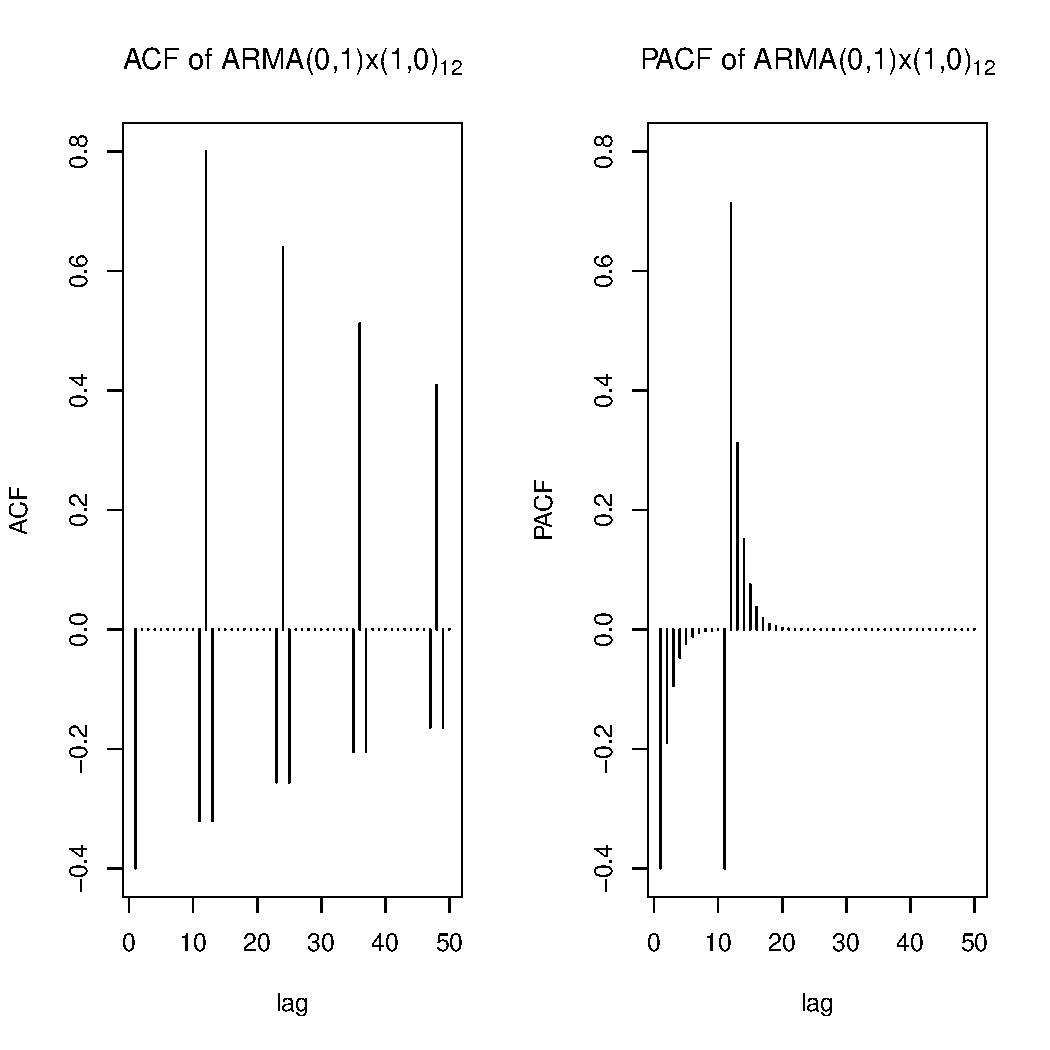
\includegraphics[width=100mm, height=80mm]{arma_acf.pdf}

\end{frame}


\begin{frame}
\frametitle{Next...}

Next we will look at removing seasonal non-stationarity and the full SARIMA model.

\end{frame}

\end{document} 